\documentclass[letterpaper, 10 pt, journal, twoside]{IEEEtran}
% \input{archive/main.config.tex}
\usepackage[maxnames=6,firstinits=true,doi=false,url=true,isbn=false]{biblatex}
% \addbibresource{IROS.bib}
\addbibresource{cav_tg.bib}
\usepackage{array}
\usepackage{graphicx}
\usepackage{amsmath}
\usepackage{amssymb}
\usepackage{color}
\usepackage{threeparttable}
\usepackage{balance} %balance columns
\hyphenation{op-tical net-works semi-conduc-tor}
\usepackage{enumitem}
\usepackage{hyperref} % Add  [ocgcolorlinks,pdfusetitle] before hyperref for colored links
% \usepackage{subfig}
\usepackage{subcaption}
\usepackage{dblfloatfix}
\usepackage{booktabs}
\usepackage{authblk}
\newcommand{\TODO}[1]{{\color{red}\textbf{TODO: #1}}}
% \pagenumbering{gobble} %suppresses page numbers
\usepackage{balance} %balance columns
% \usepackage{todonotes}
\usepackage[disable]{todonotes}
\usepackage{siunitx}
% \usepackage{draftwatermark}

%-------------------------------------------------------------------------------

\begin{document}

% ***************************************************
%  TITLE
% ***************************************************
\title{Test Generation Methods for Verification of Autonomous Systems}

\author{Kerstin Eder, Abanoub Ghobrial, Greg Chance, Severin Lemaignan, Tony Pipe  
\thanks{{\footnotesize
Manuscript  
received ...;
revised ...;  
accepted.... 
Date of publication ...;
date of current version ....

This research has in part been funded by the ROBOPILOT, CAPRI and CAVFOURTH projects. Both projects are part-funded by the Centre for Connected and Autonomous Vehicles (CCAV), delivered in partnership with Innovate UK under grant numbers 103703 (CAPRI) 103288 (ROBOPILOT) and 000000 (CAVFOURTH), respectively.
The Associate Editor for this paper was ....(\textit{Corresponding author: ....})

A.Ghobrial (e-mail: abanoub.ghobrial@bristol.ac.uk), 
G.Chance (e-mail: greg.chance@bristol.ac.uk), 
K.McAreavey (e-mail: kevin.mcareavey@bristol.ac.uk), 
and 
K.Eder (e-mail: kerstin.eder@bristol.ac.uk) 
are with the Trustworthy Systems Lab, Department of Computer Science, University of Bristol, Merchant Ventures Building, Woodland Road,  Bristol, BS8 1UQ, United Kingdom. 

S.Lemaignan (e-mail: severin.lemaignan@brl.ac.uk)
and
T.Pipe (e-mail: tony.pipe@brl.ac.uk), 
are with the Bristol Robotics Lab, T Block, University of the West of England,Frenchay, Coldharbour Ln, Bristol, BS34 8QZ, United Kingdom. 

Digital Object Identifier ....
}}}
\affil{Trustworthy Systems Laboratory, University of Bristol, Bristol, UK}
\affil{University of West of England, Bristol, UK}
\affil{Bristol Robotics Laboratory, Bristol, UK}

\markboth{IEEE TRANSACTIONS ON INTELLIGENT TRANSPORTATION SYSTEMS VOL. ..., NO. ..., date...}{Ghobrial \MakeLowercase{\textit{et al.}}: On Determinism of Game Engines used for Simulation-based Autonomous Vehicle Verification}

\maketitle
%
\begin{abstract}
\noindent 
Test generation...
        
\end{abstract}

\begin{IEEEkeywords}
Verification, Test Generation, Autonomous Vehicles, Simulation, Testing
\end{IEEEkeywords}
\IEEEpeerreviewmaketitle

% ***************************************************
%  INTRODUCTION
% ***************************************************
\section{Introduction} \label{s:introduction}

\IEEEPARstart{S}{}imulation-based verification...

\begin{figure}[!b]
    \centering
    \begin{subfigure}{.48\textwidth}
        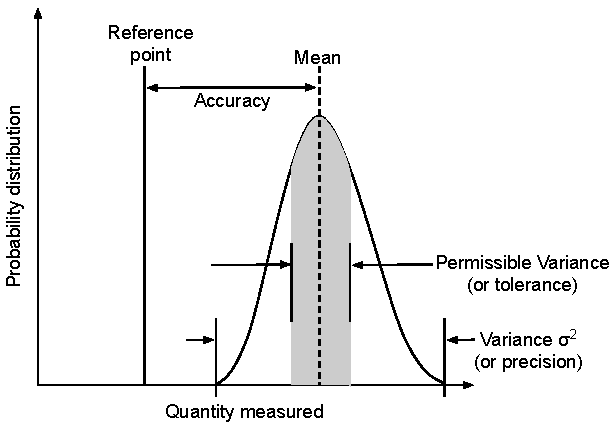
\includegraphics[width=1\textwidth]{Figures/Variance_predicition_tolerance_definition_diagram_a.pdf}
        \caption{Non-deterministic}
        \label{variance_description_a}
    \end{subfigure}
\end{figure}



% ***************************************************
%  CONCLUSION
% ***************************************************
\section{Conclusions \& Future Work}\label{s:conclusion}



% ***************************************************
%  FUNDING, REFS
% ***************************************************
% \section*{Acknowledgements}
% This research has in part been funded by the ROBOPILOT and CAPRI projects. Both
% projects are part-funded by the Centre for Connected and Autonomous
% Vehicles (CCAV), delivered in partnership with Innovate UK under grant numbers
% 103703 (CAPRI) and 103288 (ROBOPILOT), respectively.
\printbibliography

\end{document}
